\subsection{Astrophysik}
\label{subsec:astro}
Es ist ein warmer Sommerabend und du bist mit deinen Freunden am Strand oder in einem Park unterwegs und ihr schaut euch die Sterne an. Während alle anderen nur das romantische Bild des Himmels genie\ss en, überlegst du dir, wie weit der Stern ganz im Süden wohl ist, ob es überhaut ein Stern oder doch ein Plantet ist, was in seinem Inneren vorgeht? Wenn dir diese Situation bekannt vorkommt, ist \fach{Astronomie} als Nebenfach das Richtige für dich. Hier lernt man, das Universum physikalisch zu verstehen. Das bedeutet, es ist kein Nebenfach für reine Sterngucker, die möglichst viele hübsche bunte Bilder sehen wollen (keine Angst, die gibt es aber natürlich auch), sondern man beschäftigt sich mit Strahlungsprozessen, den Geschehnissen in unserer Sonne und unserem Planetensystem. Gerade das Kapitel Strahlung wirkt zu Beginn leicht abschreckend, stellt aber nach anfänglichen Schwierigkeiten kein grö\ss eres Problem dar.\\
Mit \fach{Astronomie} als Nebenfach könnt ihr bis zu 25 CP's sammeln und damit sogar die 22 CP, die ihr maximal für den Bachelor braucht, abdecken. Dabei ist es in zwei Module aufgeteilt: Das erste Modul, welches euch 12 CP gibt, besteht aus zwei Vorlesungen, die ihr ohne Probleme in den ersten beiden Semestern hören könnt. Dort werdet ihr euch vor allem mit der Sternentwicklung, Planetensystemen, unserer Sonne und Galaxien beschäftigen. Im zweiten Modul müsst ihr eine Spezialvorlesung hören und an einem Praktikum sowie einem Seminar teilnehmen. Im Allgemeinen kann man das Praktikum, welches nur im Sommersemester angeboten wird, schon im 2. Semester machen, da die einzige Voraussetzung die \VL{Astro1} Vorlesung ist. Somit könnt ihr mit eurem Nebenfach nach dem 3. Semester fertig sein, was insofern ganz praktisch ist, da man in den höheren Semestern noch Wahlpflichtveranstaltungen belegen muss, wofür man so mehr Zeit hat. Au\ss erdem ist der Praktikumsinhalt auf die 2. Vorlesung abgestimmt, ihr könnt damit also sehr leicht euer Wissen verfestigen. Zum Ende des 2. Semesters kommen nun endlich auch die Sternegucker unter euch auf ihre Kosten. Im Rahmen des Praktikums wird eine Beobachtungsnacht auf dem kleinen Feldberg veranstaltet, bei der ihr viele der von euch zuvor theoretisch untersuchten Objekte auch mal live sehen könnt. Für das Modul \Modul{AstroB} erhaltet ihr 13CP's.
%Gehalten werden alle Vorlesungen und das Praktikum von Professor T. Boller, der eigentlich am MPE, dem Max-Planck-Institut für extraterrestrische Physik in Garching bei München, arbeitet und jeweils einmal pro Woche an die Universität Frankfurt kommt.
%Dies weist den Vorteil auf, dass er an aktuellster Forschung beteiligt ist, was in der Vorlesung seinen Einfluss findet.
\von{Patricia}
\begin{figure}[!t]
 	\centering
  	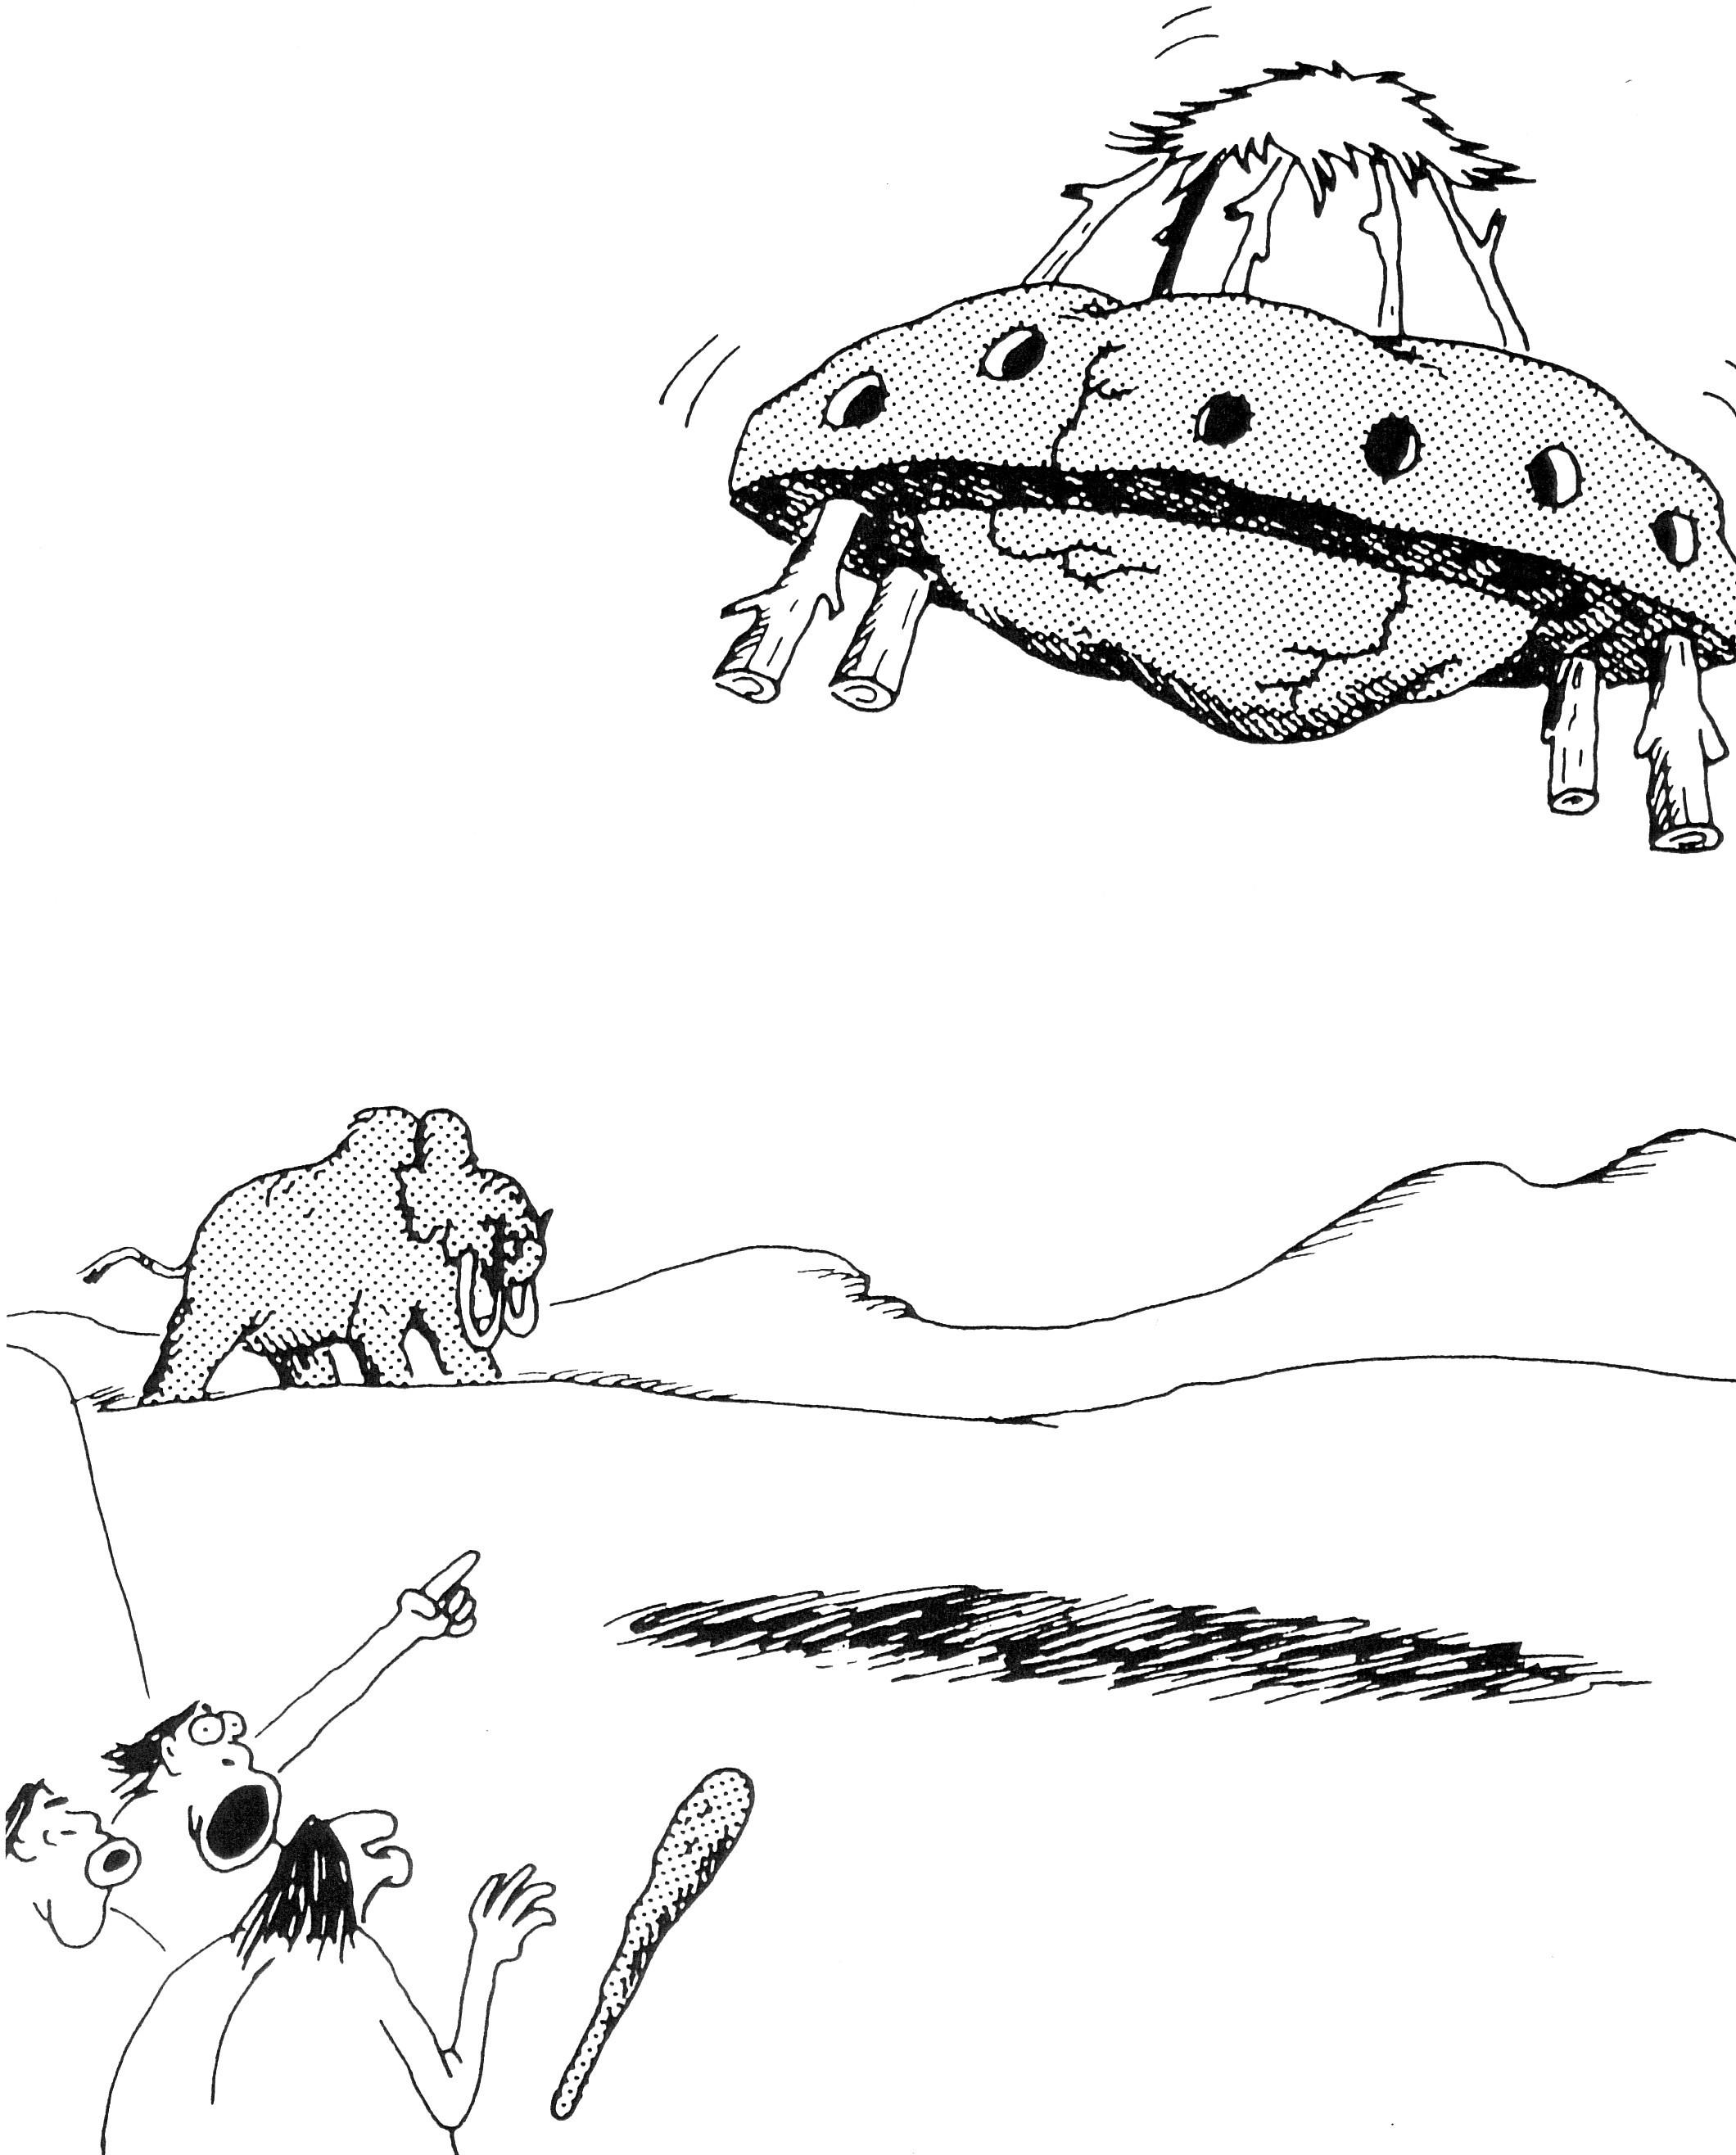
\includegraphics[width=.4\textwidth]{\imgdir/steinufo.jpg}
\end{figure}